\documentclass[12pt,a4paper]{article}

\usepackage[utf8]{inputenc}
\usepackage[T1]{fontenc}
\usepackage[brazil]{babel}
\usepackage{geometry}
\geometry{a4paper, margin=2.5cm}
\usepackage{setspace}
\onehalfspacing
\usepackage{indentfirst}
\usepackage{booktabs}
\usepackage{tabularx}
\usepackage{multirow}
\usepackage{amsmath}
\usepackage{hyperref}
\usepackage{parskip}
\setlength{\parskip}{6pt}
\usepackage{microtype}
\usepackage{caption}
\usepackage{float}
\usepackage{enumitem}
\usepackage{graphicx}
\usepackage[round]{natbib}

\title{%
  \textbf{Pseudo-rotulagem fraca para reconhecimento de entidades}\\
  \textbf{em relatos do Disque Denúncia}\\[6pt]
  \large Trabalho 3 -- Tema 6\\
  CIC1205 -- Machine Learning
}
\author{}
\date{Junho de 2026}

\begin{document}

\maketitle
\tableofcontents
\newpage

\section{Contexto e motivação}

O reconhecimento automático de entidades nomeadas (REN) em textos informais é
uma das tarefas mais desafiadoras do processamento de linguagem natural. Quando
esses textos vêm de um domínio especializado, como relatos criminais registrados
em serviços de segurança pública, as dificuldades se multiplicam: a linguagem é
repleta de abreviações, apelidos, variações ortográficas e referências locais que
raramente aparecem em corpora genéricos usados para treinar modelos padrão.

O ponto de partida deste trabalho é a dissertação de mestrado de Gustavo Melo,
que investigou o problema de REN em relatos informais do serviço Disque Denúncia
do Rio de Janeiro. O objetivo central da dissertação foi identificar automaticamente
entidades dos tipos Pessoa, Localização e Organização em textos brutos, sem
estrutura predefinida. O corpus utilizado, chamado DDsmall, contém 5.230 relatos
anotados manualmente.
Além desse corpus anotado, existe um corpus muito maior e sem anotações
manuais de REN, denominado DDlarge, com 184.493 relatos criminais. Na
dissertação, a estratégia principal para aproveitar o DDlarge foi a
pseudo-rotulagem com modelos de linguagem de grande porte, em particular o
GLiNER \citep{zaratiana2023gliner}, que avalia o contexto ao redor de cada
candidato a entidade antes de atribuir um rótulo. Essa abordagem produz
resultados expressivos, mas exige recursos computacionais consideráveis e
tempo de treinamento elevado.

Este trabalho investiga uma alternativa mais simples e interpretável: usar as
próprias entidades já anotadas no conjunto de treino como um dicionário de
entidades conhecidas e, a partir desse dicionário, marcar automaticamente as
ocorrências correspondentes nos relatos do DDlarge. Essa estratégia é conhecida
na literatura como \emph{projeção lexical} e a hipótese central é que os exemplos
adicionais gerados dessa forma podem expor o modelo a uma maior diversidade de
contextos reais, melhorando sua capacidade de generalização para entidades já
conhecidas.

\section{Conjuntos de dados}

O trabalho utilizou os mesmos corpora considerados na dissertação de Gustavo Melo:

\begin{itemize}
  \item \textbf{DDsmall}: corpus manualmente anotado, com 5.230 relatos distribuídos
    em três partições. O conjunto de treino contém 4.226 relatos, o conjunto de
    validação contém 212 relatos e o conjunto de teste contém 792 relatos. As
    anotações identificam entidades dos tipos Pessoa, Localização e Organização
    com seus respectivos spans de caracteres no texto original.
  \item \textbf{DDlarge}: corpus sem anotações manuais de REN, contendo 184.493
    relatos criminais. Esse corpus foi usado exclusivamente como fonte de
    pseudo-anotação, nunca para avaliação.
\end{itemize}

O conjunto de teste do DDsmall foi mantido completamente isolado durante todo o
desenvolvimento. Nenhuma entidade presente no teste foi usada para construir o
léxico ou calibrar qualquer parâmetro. A avaliação final dos modelos foi realizada
exclusivamente sobre esse conjunto.

Os relatos do DDsmall foram carregados a partir de arquivos JSON estruturados,
onde cada registro contém um identificador único, o texto do relato e uma lista
de spans anotados com início, fim e rótulo. O DDlarge foi processado em formato
JSONL e percorrido de forma incremental para evitar consumo excessivo de memória,
dado o volume de 184 mil registros.

\section{Entidades consideradas}

As três categorias de entidades seguem diretamente a definição adotada na
dissertação de Gustavo Melo:

\begin{itemize}
  \item \textbf{Pessoa}: nomes próprios, apelidos, alcunhas ou qualquer referência
    a indivíduos mencionados nos relatos, como ``Ruan'', ``Mara'' ou ``felipe branco''.
  \item \textbf{Localização}: bairros, ruas, comunidades, morros, logradouros,
    pontos de referência e demais expressões espaciais, como ``São Gonçalo'',
    ``favelinha'' ou ``estrada rio são Paulo''.
  \item \textbf{Organização}: instituições, órgãos públicos, unidades policiais,
    facções, empresas, plataformas ou grupos organizados, como ``polícia'',
    ``Facebook'' ou ``Batalhão''.
\end{itemize}

Essas três categorias apresentam comportamentos distintos. Localizações tendem a
ser mais frequentes e mais estáveis em termos de grafia. Pessoas concentram alta
variação lexical (apelidos informais, grafias inconsistentes) e são a categoria
com maior queda de desempenho quando a pseudo-rotulagem é aplicada. Organizações
ficam em posição intermediária, com algumas entidades muito frequentes e muitas
outras raras ou ambíguas.

\section{Metodologia}

A abordagem proposta foi dividida em cinco etapas sequenciais: extração do léxico,
filtragem, projeção lexical, construção do corpus pseudo-anotado e treinamento
dos modelos.

\subsection{Etapa 1: extração do léxico de entidades}

A primeira etapa consistiu em percorrer os 4.226 relatos do conjunto de treino
do DDsmall e registrar cada entidade anotada. Para cada ocorrência, foram
armazenados: a forma de superfície original (texto exato extraído pelo span); o
rótulo associado; a frequência total de ocorrências no treino; o conjunto de
documentos distintos em que a entidade aparece; e o conjunto de todas as formas
ortográficas distintas observadas para a mesma entidade normalizada.

A chave do índice foi a forma normalizada de cada entidade: texto em minúsculas,
sem acentos (usando decomposição Unicode NFKD com codificação ASCII) e com espaços
duplicados colapsados. Essa normalização permitiu agrupar variantes como
``polícia'' e ``policia'' sob a mesma chave, preservando cada forma de superfície
original para uso na projeção. O resultado foi um índice bruto com 5.899 entidades
únicas (contadas por chave normalizada).

\subsection{Etapa 2: normalização e filtragem do léxico}

O índice bruto foi submetido a cinco filtros sequenciais para remover entradas
com alto risco de gerar pseudo-anotações incorretas:

\begin{enumerate}
  \item \textbf{Filtro de tamanho}: entidades com menos de 3 caracteres foram
    removidas, exceto aquelas presentes em uma lista de siglas do domínio
    (\texttt{pm}, \texttt{cv}, \texttt{tcp}, \texttt{adf}, \texttt{bope},
    \texttt{pmerj}, \texttt{upa}, \texttt{upp}, \texttt{rj}, \texttt{dp},
    \texttt{br}, \texttt{pf}). Esse filtro eliminou 51 entidades, como ``sg'',
    com 15 ocorrências como Localização, ``p2'', com 15 ocorrências
    majoritariamente como Organização, e ``ph'', com 12 ocorrências como
    Pessoa. Siglas de alta frequência, como ``rj'', com 217 ocorrências, e
    ``dp'', permanecem no léxico por estarem na lista de exceções.

  \item \textbf{Filtro de termos genéricos}: palavras isoladas consideradas
    excessivamente genéricas seriam removidas do léxico caso ocorressem como
    entidade completa (não apenas como parte de uma entidade composta),
    incluindo termos como ``rua'', ``morro'', ``comunidade'', ``elementos'',
    ``bandidos'', ``area'', ``local'', ``lugar'', ``homem'', ``mulher'',
    ``beco'' e ``rodovia''. Na prática, nenhuma chave do índice bruto coincide
    exatamente com esses termos isolados. Eles aparecem nas anotações apenas
    como parte de spans maiores, como em ``rua Augusto Rush'', de modo que
    esse filtro não eliminou nenhuma entrada nesta execução.

  \item \textbf{Filtro de frequência mínima}: entidades observadas em duas ou
    menos ocorrências no treino foram descartadas. Esse filtro foi introduzido
    porque uma entidade com frequência 1 é 100\%
    dominante em sua única classe observada, mesmo quando essa observação é um
    erro de anotação ou uma palavra comum usada fora de um contexto de
    entidade (ex.: ``mão'' anotada uma única vez como Pessoa). Esse foi o
    filtro mais impactante: eliminou 4.762 entidades, sendo 3.996 com
    frequência 1 e 766 com frequência 2.

  \item \textbf{Filtro de dominância}: entidades associadas a mais de uma classe
    no treino foram mantidas apenas se uma classe representasse pelo menos 80\%
    das ocorrências. Entidades abaixo desse limiar foram descartadas por
    apresentar ambiguidade semântica. Esse filtro eliminou 29 entidades, como
    ``flamengo'', com 6 ocorrências como Organização e 16 como Localização,
    uma dominância de apenas 72,7\%, e ``botafogo'', com 9 ocorrências como
    Localização, 7 como Organização e 2 como Pessoa, sem classe claramente
    dominante.

  \item \textbf{Filtro de rótulo válido}: apenas entidades cuja classe dominante
    fosse uma das três válidas, Pessoa, Localização ou Organização, foram mantidas.
\end{enumerate}

Ao final da filtragem, o léxico contou com 1.057 entidades válidas: 662
Localizações (62,6\%), 248 Pessoas (23,5\%) e 147 Organizações (13,9\%). Essa
filtragem representou uma redução de 82,1\% em relação ao índice bruto,
decorrente majoritariamente do filtro de frequência mínima.

A Figura~\ref{fig:freq_hist} mostra a distribuição de frequência das entidades
antes e depois da filtragem, em escala logarítmica. O índice bruto, com 5.899
entidades, tem mediana de frequência 1 e média 2,72. A maioria das entidades
aparece em um único relato do treino. Após a filtragem, a mediana sobe para 5
e a média para 9,65, mantendo o máximo de 600 ocorrências para ``polícia'',
evidenciando que o léxico resultante é composto por entidades com evidência
estatística bem mais robusta.

\begin{figure}[H]
\centering
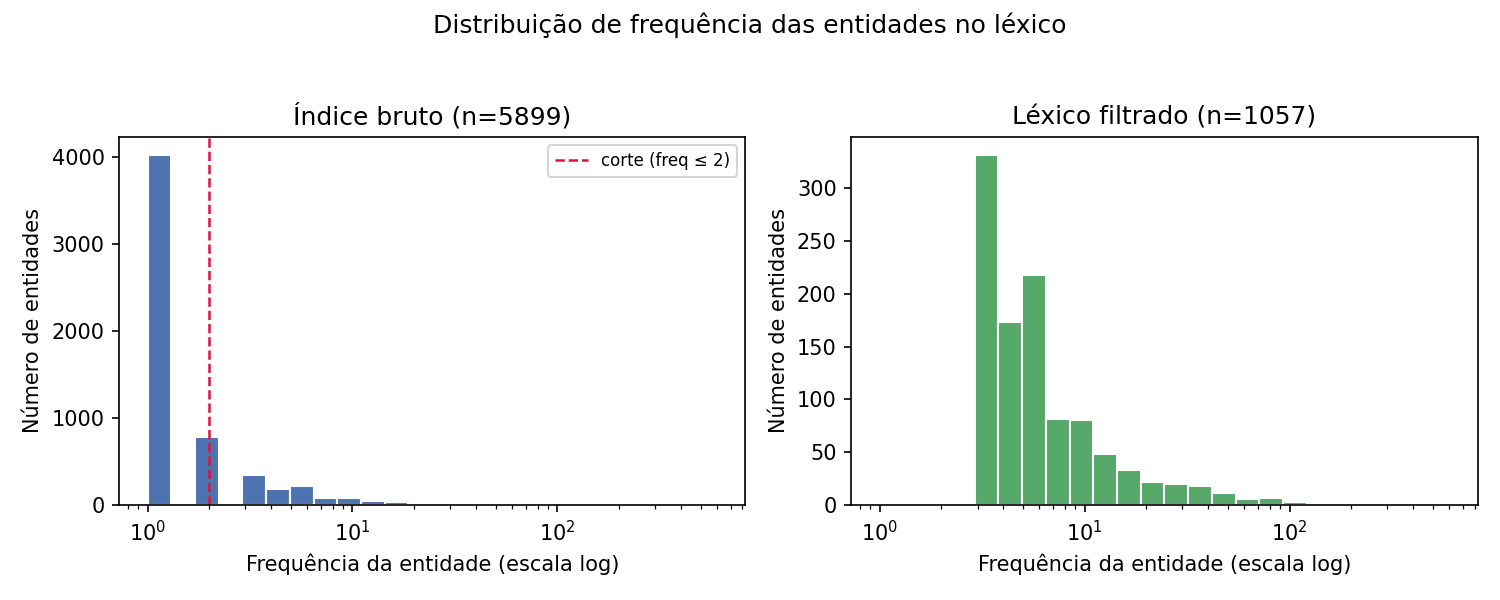
\includegraphics[width=\textwidth]{figuras/freq_histograma.png}
\caption{Distribuição de frequência das entidades no índice bruto (esquerda)
e no léxico filtrado (direita), em escala logarítmica. A linha pontilhada
marca o corte do filtro de frequência mínima.}
\label{fig:freq_hist}
\end{figure}

\subsection{Etapa 3: projeção lexical sobre o DDlarge}

A projeção lexical buscou, nos relatos do DDlarge, ocorrências das entidades do
léxico filtrado. Para isso, foi utilizado o \texttt{PhraseMatcher} da biblioteca
spaCy com o atributo \texttt{LOWER}, que realiza casamento insensível a
maiúsculas e minúsculas com base em tokens. O uso de tokens, em vez de busca
por substring bruta, garante o respeito a fronteiras de palavra.

Internamente, o PhraseMatcher utiliza uma estrutura de busca baseada em trie,
adaptada do algoritmo FlashText \citep{singh2017flashtext}, para realizar a correspondência
simultânea de grandes conjuntos de expressões. Essa abordagem permite localizar múltiplos
padrões em uma única passagem pelo texto, mantendo bom desempenho mesmo quando
milhares de termos são registrados. Essa característica viabilizou, com custo computacional reduzido, a projeção sobre os 184 mil relatos do DDlarge: o PhraseMatcher foi construído uma única vez com as 1.057 entidades do léxico filtrado antes do processamento dos registros. Para cada entidade, todas as formas observadas no conjunto de treino foram registradas como padrões distintos sob o mesmo rótulo.

A resolução de sobreposições seguiu a regra de preferir o span mais longo: quando
dois spans se sobrepõem, o de maior comprimento é mantido e o mais curto é
descartado. Isso evita que entidades compostas sejam fragmentadas em componentes
menores. Empates de comprimento foram resolvidos pela posição mais à esquerda
no texto.

\subsection{Etapa 4: construção do corpus pseudo-anotado}

Dos 184.493 relatos do DDlarge, 133.841 receberam pelo menos uma pseudo-anotação
(72,5\% do corpus). O total de pseudo-entidades geradas foi 450.833: 236.763
Localizações (52,5\%), 142.636 Organizações (31,6\%) e 71.434 Pessoas (15,8\%).

Uma inspeção manual de amostras revelou tanto casos plausíveis quanto casos
suspeitos. Entre os plausíveis: ``São Gonçalo'', ``Guaxindiba'' e ``Jardim
Catarina'' marcadas como Localização em relatos com contexto espacial
coerente, e ``upp'' como Organização ao se referir a uma unidade policial.
Entre os suspeitos estão ``posse'' marcada como Localização no trecho ``mesmo
com upp na região os meliantes praticam assaltos [...] em posse de'', um
substantivo comum confundido com o topônimo homônimo do léxico, e
``PROVIDENCIA'' como Localização em contextos que não se referem ao Morro da
Providência. A projeção também fragmenta entidades compostas que não estão
registradas como tal no léxico: no relato ``Dodô, felipe branco, e Sandro são
alguns que comandam [...]'', o apelido ``felipe branco'' foi anotado como
dois spans de Pessoa separados, ``felipe'' e ``branco'', porque o léxico
contém as duas palavras isoladamente, mas não a forma composta. O filtro de
frequência mínima da Etapa 2 não é suficiente para eliminar casos como
``posse'' e ``PROVIDENCIA'', cuja frequência no treino, 4 e 5 respectivamente,
é alta o bastante para superar o filtro mesmo sendo ambíguos. Esses casos
ilustram a limitação estrutural da projeção lexical: ela não avalia o
contexto ao redor da ocorrência.

\subsection{Etapa 5: treinamento dos modelos}

Todos os modelos treinados do zero utilizaram a biblioteca spaCy com um pipeline
em branco para o português (\texttt{spacy.blank('pt')}), ao qual foi adicionado
o componente de NER treinável. Os exemplos de treinamento foram construídos
convertendo cada registro anotado em um objeto \texttt{Example} do spaCy,
associando o texto original aos spans anotados. O treinamento foi executado com
semente aleatória fixada em 42. Para a Proposta 2, os exemplos do DDsmall e os
pseudo-exemplos do DDlarge foram combinados e embaralhados antes do treinamento.

\section{Modelos e configurações experimentais}

Foram comparadas cinco configurações:

\begin{description}
  \item[Baseline 1 (zero-shot)] O modelo pré-treinado \texttt{pt\_core\_news\_lg}
    do spaCy, aplicado diretamente ao conjunto de teste sem adaptação ao domínio.
    Os rótulos originais (PER, LOC, ORG) foram mapeados para os rótulos do
    DDsmall (Pessoa, Localização, Organização).

  \item[Proposta 1 (EntityRuler)] Sistema baseado puramente em regras, construído
    com o componente \texttt{EntityRuler} do spaCy. Para cada entidade do léxico,
    cada forma de superfície foi registrada como um padrão, com casamento
    insensível a maiúsculas. Os padrões foram ordenados do mais longo para o
    mais curto.

  \item[Baseline 2 (DDsmall)] Modelo NER treinado exclusivamente com os 4.226
    relatos do conjunto de treino do DDsmall. Representa o desempenho alcançável
    com a anotação manual disponível, sem dados adicionais.

  \item[Proposta 2 (20k pseudo)] Modelo NER treinado com os 4.226 relatos do
    DDsmall combinados com os primeiros 20.000 relatos pseudo-anotados do DDlarge.

  \item[Proposta 2 (completo)] Variante que utilizou todos os 133.841 relatos
    pseudo-anotados do DDlarge combinados com os 4.226 relatos do DDsmall.
\end{description}

\section{Métricas de avaliação}

A avaliação foi realizada no nível de entidade: uma predição é correta somente
quando o span de início e fim coincide exatamente com a anotação de referência
e o rótulo de classe também é correto. Foram reportadas precisão, revocação e
F1 por classe, F1 micro, que soma os totais globais de TP, FP e FN, e F1
macro, a média simples entre as três classes.

\begin{table}[H]
\centering
\caption{Avaliação em nível de entidade no conjunto de teste do DDsmall.
Uma predição é correta somente quando span e classe coincidem exatamente.}
\label{tab:entidade}
\small
\begin{tabular}{lrrrrrrrrrr}
\toprule
& \multicolumn{3}{c}{\textbf{Pessoa}} & \multicolumn{3}{c}{\textbf{Localização}} & \multicolumn{3}{c}{\textbf{Organização}} & \\
\cmidrule(lr){2-4}\cmidrule(lr){5-7}\cmidrule(lr){8-10}
\textbf{Modelo} & P & R & F1 & P & R & F1 & P & R & F1 & \textbf{micro-F1} \\
\midrule
Baseline 2 (DDsmall)    & 0,749 & 0,722 & 0,735 & 0,834 & 0,828 & 0,831 & 0,749 & 0,750 & 0,749 & \textbf{0,795} \\
Proposta 2 (20k)        & 0,589 & 0,441 & 0,504 & 0,815 & 0,658 & 0,729 & 0,692 & 0,691 & 0,692 & 0,676 \\
Proposta 1 (EntityRuler)& 0,552 & 0,406 & 0,468 & 0,830 & 0,591 & 0,690 & 0,687 & 0,671 & 0,679 & 0,642 \\
Proposta 2 (completo)   & 0,535 & 0,398 & 0,457 & 0,828 & 0,596 & 0,693 & 0,723 & 0,640 & 0,679 & 0,641 \\
Baseline 1 (zero-shot)  & 0,408 & 0,495 & 0,447 & 0,409 & 0,347 & 0,375 & 0,254 & 0,149 & 0,187 & 0,362 \\
\bottomrule
\end{tabular}
\end{table}

O Baseline 2 obteve o melhor desempenho, com micro-F1 de 0,795. A melhor
variante da Proposta 2, a de 20k, ficou em segundo lugar, com queda de 11,9
pontos percentuais. A Proposta 1, baseada puramente em regras, alcançou 0,642,
ficando praticamente empatada com a Proposta 2 completa, que obteve 0,641 ao
usar todos os 133.841 relatos pseudo-anotados em vez de apenas 20 mil. Isso
sugere que ampliar a quantidade de pseudo-exemplos não trouxe ganho adicional
depois que a Proposta 2 já supera o teto de um sistema de regras puro. O
Baseline 1, zero-shot, ficou bem atrás de todas as demais configurações, com
micro-F1 de 0,362.

\section{Análises}

\subsection{Análise do léxico}

\begin{table}[H]
\centering
\caption{Visão geral do léxico extraído do conjunto de treino.}
\label{tab:lexico}
\begin{tabular}{lr}
\toprule
\textbf{Medida} & \textbf{Valor} \\
\midrule
Entidades brutas (formas normalizadas únicas)         & 5.899 \\
Entidades após filtragem                              & 1.057 \\
Entidades removidas                                   & 4.842 \\
\quad Por tamanho muito pequeno (${<}$3 caracteres)    &    51 \\
\quad Por frequência mínima (freq $\leq$ 2)            & 4.762 \\
\quad Por ambiguidade de classe (dominância $<$ 80\%)  &    29 \\
\midrule
Localizações no léxico filtrado                       &   662 \\
Pessoas no léxico filtrado                            &   248 \\
Organizações no léxico filtrado                       &   147 \\
\midrule
Frequência mediana (léxico filtrado)                  &     5 \\
Frequência média (léxico filtrado)                    &  9,65 \\
Frequência máxima (``polícia'')                       &   600 \\
\bottomrule
\end{tabular}
\end{table}

No índice bruto, a distribuição de frequência é fortemente concentrada em
valores baixos, com mediana 1, conforme mostra a Figura~\ref{fig:freq_hist}
apresentada na Etapa 2: a maioria das entidades aparece em apenas um relato
do treino. O filtro de frequência mínima desloca essa distribuição no léxico
final, cuja mediana sobe para 5. A entidade mais frequente, ``polícia'',
aparece 600 vezes como Organização. Entre as demais entidades frequentes
estão ``São Gonçalo'', com 192 ocorrências como Localização, ``favelinha'',
com 155, ``Tijuca'', com 137, ``Rio de Janeiro'', com 101, ``Facebook'', com
100 ocorrências como Organização, e ``pm'', com 86.

Entre as entidades removidas, os casos mais representativos são ``sg'',
removida pelo filtro de tamanho, ``Fernando beira mar'', removida pelo filtro
de frequência mínima com apenas 2 ocorrências como Pessoa, e ``Ipase'',
removida por ambiguidade: 4 ocorrências como Localização e 2 como
Organização, dominância de apenas 67\%.

\subsection{Análise das pseudo-anotações}

Dos 184.493 relatos do DDlarge, 133.841 receberam pelo menos uma pseudo-anotação,
correspondendo a 72,5\% do corpus. O total de 450.833 pseudo-entidades se
distribui em 236.763 Localizações (52,5\%), 142.636 Organizações (31,6\%) e
71.434 Pessoas (15,8\%), proporção próxima à observada no léxico filtrado.

A inspeção manual confirmou tanto casos plausíveis quanto suspeitos. Casos
plausíveis incluem menções geográficas bem definidas como ``São Gonçalo'',
``Guaxindiba'' e ``Jardim Catarina'' marcadas como Localização em contextos
espaciais coerentes. Casos suspeitos incluem ``posse'' marcado como
Localização em ``[...] os meliantes praticam assaltos [...] em posse de'' e
``PROVIDENCIA'' como Localização em contextos que não se referem ao Morro da
Providência. Há também fragmentação de entidades compostas que não estão
registradas como tal no léxico: ``felipe branco'' aparece anotado como dois
spans de Pessoa separados (``felipe'' e ``branco'').

Esses erros não podem ser detectados pela projeção lexical sem uso de contexto,
e representam ruído sistemático no corpus pseudo-anotado.

\subsection{Análise qualitativa de erros}

A comparação central é entre o Baseline 2 e a Proposta 2 (20k). A
Tabela~\ref{tab:erros} apresenta os contadores de cada categoria de erro.

\begin{table}[H]
\centering
\caption{Contagem de erros por categoria para o Baseline 2 e a Proposta 2 (20k).
Acertos exatos não entram na contagem.}
\label{tab:erros}
\small
\begin{tabular}{lrr}
\toprule
\textbf{Categoria de erro} & \textbf{Baseline 2} & \textbf{Proposta 2 (20k)} \\
\midrule
Falso negativo / fora do léxico              & 188 & 557 \\
Falso negativo / variação ortográfica        &  68 & 219 \\
Erro de fronteira / composta parcial         & 110 & 217 \\
Falso positivo (puro)                        & 264 & 296 \\
Erro de fronteira / span maior               & 109 &  52 \\
Erro de classe                               & 119 &  83 \\
Falso negativo / no léxico, não reconhecida  &  42 &  33 \\
Erro de fronteira / deslocado                &   3 &   2 \\
\bottomrule
\end{tabular}
\end{table}

\subsubsection{Falsos negativos fora do léxico}

Essa é a categoria que mais cresceu em termos absolutos, saltando de 188 para
557, um aumento de 196\%. Como o léxico filtrado ficou bem menor depois do
filtro de frequência mínima da Etapa 2, muitas entidades legítimas do DDlarge
simplesmente nunca chegaram a ser pseudo-anotadas, e o modelo nunca viu
exemplos delas durante o treinamento. Casos típicos incluem ``supermercado
vianense'', ``IMPRENSA'' e ``Colubandê'' classificadas como Organização ou
Localização no conjunto de teste, mas ausentes do léxico usado para gerar o
pseudo-corpus. Esse padrão aponta para uma queda de cobertura, não para ruído:
o modelo da Proposta 2 ficou mais conservador, deixando de reconhecer
entidades que o Baseline 2 já identificava corretamente.

\subsubsection{Falsos negativos por variação ortográfica}

Essa categoria mais que triplicou, de 68 para 219. Casos típicos incluem
``Adriano'' não reconhecido porque o léxico contém ``adriana'', ``Alexander''
não reconhecida porque o léxico contém ``alexandre''. O pseudo-corpus reforça as
formas exatas do léxico, e como o léxico agora cobre menos variantes
ortográficas de cada entidade, o modelo ficou mais rígido diante de grafias
que não apareceram no treino.

\subsubsection{Entidades compostas reconhecidas parcialmente}

O erro de fronteira do tipo ``composta parcial'' quase dobrou, de 110 para
217. Exemplos incluem ``morro do canta galo'' reduzido a ``canta galo'',
``estrada rio são Paulo'' reduzido a ``rio'' e ``ponta da ilha'' reduzido a
``ilha''. A projeção tende a casar sub-strings frequentes do léxico,
fragmentando entidades compostas cuja forma completa tem menor frequência do
que seus componentes isolados.

\subsubsection{Falsos positivos}

Os falsos positivos cresceram pouco, de 264 para 296, um aumento de 12\%. O
filtro de frequência mínima do léxico, descrito na Etapa 2, descarta
entidades raras antes que elas cheguem ao pseudo-corpus, o que limita a
quantidade de termos ambíguos disponíveis para gerar ruído. Os casos que
restam incluem ``providência'' marcado como Localização e ``polimix''
marcado como Organização, ambos termos que permanecem no léxico com
frequência alta o suficiente para escapar do filtro. Essa categoria não é o
principal fator de degradação da Proposta 2: as duas categorias de falso
negativo discutidas acima, fora do léxico e variação ortográfica, têm impacto
muito maior no total de erros.

\subsubsection{Erros de classe e entidades no léxico não reconhecidas}

Essas duas categorias, junto com o erro de fronteira do tipo ``span maior'',
foram as únicas em que a Proposta 2 melhorou. Os erros de classe caíram de
119 para 83, e as entidades do léxico não reconhecidas pelo modelo caíram de
42 para 33. Exemplos de erro de classe incluem ``TOP SHOPPING'' classificado
como Organização quando o gabarito é Localização, e ``marinha'' classificado
como Localização quando o gabarito é Organização. Essas melhorias sugerem que,
para as entidades que de fato chegam a ser pseudo-anotadas, ver mais contextos
ajuda o modelo a desambiguar a classe correta. O problema é que esse ganho é
pequeno demais para compensar o aumento muito maior nas duas categorias de
falso negativo.

\section{Cuidados metodológicos}

Os principais cuidados metodológicos adotados foram os seguintes. O léxico foi
extraído exclusivamente dos 4.226 relatos do treino, sem acesso ao conjunto de
teste. O conjunto de validação foi usado apenas para monitorar o treinamento e
não influenciou a construção do léxico nem os limiares de filtragem. Todos os
cinco modelos foram avaliados no mesmo conjunto de teste. A resolução de sobreposições
na projeção foi determinística (span mais longo), evitando não-determinismo
na geração do pseudo-corpus. Todas as sementes aleatórias foram fixadas em 42,
tornando os resultados reprodutíveis. Os offsets de início e fim dos spans foram
preservados em relação ao texto original, sem remapeamento.

\section{Conclusões}

Este trabalho investigou se a projeção lexical de entidades anotadas no conjunto
de treino sobre um corpus maior e não anotado pode melhorar o desempenho de
modelos leves de REN em relatos criminais informais. A hipótese não foi
confirmada: em todas as configurações testadas, os modelos treinados com
pseudo-rótulos ficaram abaixo do baseline treinado apenas com o corpus anotado
manualmente.

A análise de erros aponta para uma tensão entre precisão e cobertura no
léxico usado na projeção. O filtro de frequência mínima da Etapa 2 descarta
qualquer entidade observada em até duas ocorrências no treino, reduzindo o
índice bruto de 5.899 para as 1.057 entidades do léxico final. Essa exigência
de evidência estatística limita a quantidade de termos ambíguos disponíveis
para gerar ruído no pseudo-corpus: os falsos positivos da Proposta 2
cresceram apenas 12\% sobre o Baseline 2, de 264 para 296. Em compensação, o
léxico final cobre uma fração pequena das formas de entidade que aparecem no
DDlarge, e isso aparece nos dois tipos de falso negativo que dominam o
aumento total de erros: entidades fora do léxico, que quase triplicaram, de
188 para 557, e variantes ortográficas não cobertas pelas formas de
superfície registradas, que também mais que triplicaram, de 68 para 219.

Essa tensão é consequência direta da limitação estrutural da projeção
lexical: ela decide marcar ou não uma ocorrência apenas com base na
correspondência exata de string, sem avaliar o contexto ao redor. Um léxico
mais permissivo aumentaria a cobertura, mas também aumentaria o risco de
marcar termos ambíguos fora de contexto, como ``mão'' ou ``preto'' usados
como substantivo comum em vez de apelido, conforme discutido na Etapa 2. Um
léxico mais restrito, como o usado neste trabalho, reduz esse risco, mas
deixa de cobrir entidades raras e variantes ortográficas legítimas. As poucas
categorias em que a Proposta 2 melhorou sobre o Baseline 2, erro de classe e
entidades do léxico não reconhecidas, mostram que ver mais contextos ajuda o
modelo a desambiguar quando a entidade chega a ser pseudo-anotada, mas esse
ganho é pequeno demais para compensar o aumento nas duas categorias de falso
negativo. O contraste com a estratégia da dissertação de Gustavo Melo é
revelador: o modelo GLiNER, que avalia o contexto ao redor de cada span
candidato antes de decidir o rótulo, não depende desse compromisso entre
precisão e cobertura.

Os resultados também mostram que ampliar o volume de pseudo-exemplos não traz
ganho adicional: a variante com o corpus completo, usando 133.841 relatos,
obteve micro-F1 de 0,641, abaixo da variante com apenas 20 mil relatos
(0,676) e praticamente empatada com a Proposta 1, o sistema de regras puro
(0,642). Isso sugere que o teto de desempenho da projeção lexical está mais
ligado à qualidade e à cobertura do léxico do que à quantidade de relatos
pseudo-anotados usados no treinamento.

\bibliographystyle{apalike}
\bibliography{referencias}

\end{document}